\chapter{Implementations}
In this chapter we dive into the implementation part and discuss different approaches. First, we specify how the AFs we run the experiments on were created in \cref{sec:ImplementationsCreatingAFs}. Here we describe three different methods, with their advantages and disadvantages. In \cref{sec:ImplementationUsageAndSettings} we describe the usage of the implemented tool and the settings to change the inner workings of the algorithms.

\section{Generating AFs}
\label{sec:ImplementationsCreatingAFs}
We created three different approaches to generate AFs. Each of them has a different idea and generates AFs with different properties. While the random-based approach generates AFs, which are typically not similar to real-world problems, the grid-based approach has more structure. The level-based approach has even more structure and assures that we can not derive too many neighbours from a problematic argument. For each approach, we provide an additional figure for better visualization and example AFs generated with the algorithm.

\paragraph{Random-based} Let us begin with the random-based approach. The arguments of the script are \texttt{<arg\_amount>} and \texttt{<p>}. The \texttt{<arg\_amount>} specifies how many arguments the AF has and the argument \texttt{<p>} defines the probability of an attack between two arguments. Basically, if we take a look at \cref{fig:LevelBasedApproach} we can see a graph with potential attacks depicted with dotted arrows. Every potential attack has a a probability of \texttt{<p>} to be an actual attack of the generated AF.


\begin{figure}[h!]
    \centering
    \begin{tikzpicture}
        \def \rectSize{0.7cm}
        \def \rectSpace{1.8cm}
        \def \rectCircleAdaption{0.1cm}
        
        \node[circle, draw, line width=0.3mm, minimum width=\rectSize, minimum height=\rectSize] at (0, 0) {};
        \node[circle, draw, line width=0.3mm, minimum width=\rectSize, minimum height=\rectSize] at (\rectSpace, 0) {};
        \node[circle, draw, line width=0.3mm, minimum width=\rectSize, minimum height=\rectSize] at (0, \rectSpace) {};
        \node[circle, draw, line width=0.3mm, minimum width=\rectSize, minimum height=\rectSize] at (\rectSpace, \rectSpace) {};

        % bottom
        \draw[dotted,<->, line width=0.3mm, >={To[length=4, width=5]}]
        (0 + \rectSize/2, 0) -- (\rectSpace - \rectSize/2, 0);
        % top
        \draw[dotted,<->, line width=0.3mm, >={To[length=4, width=5]}]
        (0 + \rectSize/2, \rectSpace) -- (\rectSpace - \rectSize/2, \rectSpace);
        % left
        \draw[dotted,<->, line width=0.3mm, >={To[length=4, width=5]}]
        (0,0 + \rectSize/2) -- (0, \rectSpace - \rectSize/2);
        % right
        \draw[dotted,<->, line width=0.3mm, >={To[length=4, width=5]}]
        (\rectSpace, 0 + \rectSize/2) -- (\rectSpace , \rectSpace - \rectSize/2);
        % center positive
        \draw[dotted,<->, line width=0.3mm, >={To[length=4, width=5]}]
        (0 + \rectSize/2 - \rectCircleAdaption, 0 + \rectSize/2 - \rectCircleAdaption) -- (\rectSpace - \rectSize/2 + \rectCircleAdaption, \rectSpace-\rectSize/2 + \rectCircleAdaption);
        % center negative
        \draw[dotted,<->, line width=0.3mm, >={To[length=4, width=5]}]
        (0 + \rectSize/2-\rectCircleAdaption, \rectSpace - \rectSize/2+\rectCircleAdaption) -- (\rectSpace - \rectSize/2+\rectCircleAdaption, \rectSize/2-\rectCircleAdaption);

    \end{tikzpicture}
    \caption{Random-based approach with $Amount=4$ and $p=1$}
    \label{fig:LevelBasedApproach}
\end{figure}

Random-based generated AFs have the property (depending on the probability value) of being hard to to predict on how good the AF is solvable. This is due the fact, that the neighbours of each argument are highly dependent on the amount of attacks and randomness (since an argument can attack every other arguments). Example AFs generated with the random-based approach can be seen in \cref{fig:ImplementationRandomBasedExampleAFs}


\vspace{0.3cm}
\begin{figure}[h]
    \centering
    \begin{subfigure}[t]{0.3\textwidth}
        \centering
        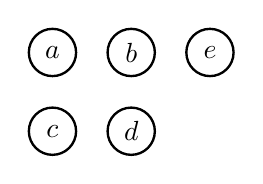
\begin{tikzpicture}
            \def \ax{0}   \def \ay{0}
            \def \bx{1}   \def \by{0}
            \def \cx{0}   \def \cy{-1}
            \def \dx{1}   \def \dy{-1}
            \def \ex{2}   \def \ey{0}

            \draw[line width=0.3mm] (\ax, \ay) circle (0.3) node[anchor=center]{$a$};
            \draw[line width=0.3mm] (\bx, \by) circle (0.3) node[anchor=center]{$b$};
            \draw[line width=0.3mm] (\cx, \cy) circle (0.3) node[anchor=center]{$c$};
            \draw[line width=0.3mm] (\dx, \dy) circle (0.3) node[anchor=center]{$d$};
            \draw[line width=0.3mm] (\ex, \ey) circle (0.3) node[anchor=center]{$e$};
            % Attacks
            \DrawSelfAttackRightSingleton{\ex}{\ey}
            \DrawAttackVertical{B}{\ax}{\ay}{\cx}{\cy}
            \DrawAttackHorizontal{R}{\ax}{\ay}{\bx}{\by}
            \DrawAttackHorizontal{L}{\dx}{\dy}{\cx}{\cy}
            \DrawAttackDiagonal{PLR}{\cx}{\cy}{\bx}{\by}
    
        \end{tikzpicture}
        \subcaption{\texttt{arg\_amount}=5 \texttt{p}=0.25}
        \label{af:ImplementationRandomBasedExampleAFsa}
    \end{subfigure}
    \begin{subfigure}[t]{0.3\textwidth}
    \centering
    \begin{tikzpicture}
        % Singletons
        \def \ax{0}   \def \ay{0}
        \def \bx{1}   \def \by{0}
        \def \cx{1}   \def \cy{-1}
        \def \dx{2}   \def \dy{0}
        \def \ex{2}   \def \ey{-1}

        \draw[line width=0.3mm] (\ax, \ay) circle (0.3) node[anchor=center]{$a$};
        \draw[line width=0.3mm] (\bx, \by) circle (0.3) node[anchor=center]{$b$};
        \draw[line width=0.3mm] (\cx, \cy) circle (0.3) node[anchor=center]{$c$};
        \draw[line width=0.3mm] (\dx, \dy) circle (0.3) node[anchor=center]{$d$};
        \draw[line width=0.3mm] (\ex, \ey) circle (0.3) node[anchor=center]{$e$};

        % Attacks
        \DrawSelfAttackLeftSingleton{\ax}{\ay}
        \DrawSelfAttackRightSingleton{\dx}{\dy}
        \DrawSelfAttackRightSingleton{\ex}{\ey}
        \DrawAttackHorizontal{L}{\bx}{\by}{\ax}{\ay}
        \DrawAttackHorizontal{R}{\bx}{\by}{\dx}{\dy}
        \DrawAttackHorizontal{R}{\cx}{\cy}{\ex}{\ey}
        \DrawAttackVertical{D}{\dx}{\dy}{\ex}{\ey}
        \DrawAttackVertical{D}{\bx}{\by}{\cx}{\cy}
        \DrawAttackDiagonal{NLR}{\bx}{\by}{\ex}{\ey}
        \DrawAttackDiagonal{NRL}{\cx}{\cy}{\ax}{\ay}

        % Weird Attack
        \def \argSize{0.3}
        \draw[-{To[length=4, width=5]}, line width=0.3mm]
            (\ax + \argSize/2, \ay + \argSize - 0.05) .. controls
            (\bx-0.2 , \by + \argSize + 0.2) and
            (\bx+0.2 , \by + \argSize + 0.2) ..
            (\dx - \argSize/2, \dy + \argSize - 0.05);
    \end{tikzpicture}
    \subcaption{\texttt{arg\_amount}=5 \texttt{p}=0.5}
    \label{af:ImplementationRandomBasedExampleAFsb}
\end{subfigure}%
\begin{subfigure}[t]{0.3\textwidth}
    \centering
    \begin{tikzpicture}
        % Singletons
        \def \ax{0}   \def \ay{0}
        \def \bx{1}   \def \by{0}
        \def \cx{0}   \def \cy{-1}
        \def \dx{1}   \def \dy{-1}
        \def \ex{2}   \def \ey{0}

        \draw[line width=0.3mm] (\ax, \ay) circle (0.3) node[anchor=center]{$a$};
        \draw[line width=0.3mm] (\bx, \by) circle (0.3) node[anchor=center]{$b$};
        \draw[line width=0.3mm] (\cx, \cy) circle (0.3) node[anchor=center]{$c$};
        \draw[line width=0.3mm] (\dx, \dy) circle (0.3) node[anchor=center]{$d$};
        \draw[line width=0.3mm] (\ex, \ey) circle (0.3) node[anchor=center]{$e$};

        % Attacks
        \DrawSelfAttackLeftSingleton{\ax}{\ay}
        \DrawSelfAttackLeftSingleton{\cx}{\cy}
        \DrawSelfAttackRightSingleton{\ex}{\ey}
        \DrawAttackDiagonal{NB}{\ax}{\ay}{\dx}{\dy}
        \DrawAttackDiagonal{PB}{\bx}{\by}{\cx}{\cy}
        \DrawAttackHorizontal{L}{\bx}{\by}{\ax}{\ay}
        \DrawAttackHorizontal{R}{\cx}{\cy}{\dx}{\dy}
        \DrawAttackHorizontal{L}{\ex}{\ey}{\bx}{\by}
        \DrawAttackVertical{B}{\ax}{\ay}{\cx}{\cy}

        % Weird Attack
        \def \argSize{0.3}
        \draw[-{To[length=4, width=5]}, line width=0.3mm]
            (\ax + \argSize/2, \ay + \argSize - 0.05) .. controls
            (\bx-0.2 , \by + \argSize + 0.2) and
            (\bx+0.2 , \by + \argSize + 0.2) ..
            (\ex - \argSize/2, \ey + \argSize - 0.05);
    \end{tikzpicture}
    \subcaption{\texttt{arg\_amount}=5 \texttt{p}=0.75}
    \label{af:ImplementationRandomBasedExampleAFsc}
\end{subfigure}
\caption{Example AF generated with random-based approach}
\label{fig:ImplementationRandomBasedExampleAFs}
\end{figure}
\vspace{0.3cm}



\paragraph{Grid-based} Next we are going to discuss the grid-based approach. The arguments for the script are \texttt{<arg\_amount>}, being the amount of arguments the AF has and \texttt{<p>}, which is the probability that an attack between two arguments occurs. Different to the random-based approach, attacks can only happen between the direct neighbours of the grid (i.e.\ top, bottom, right, left). The grid is an $n \times n$ grid, with $n$ being equal to $\lfloor (\sqrt{\texttt{<arg\_amount>}}) \rfloor$. An example grid can be seen in \cref{fig:GridBasedApproach}.

\begin{figure}[h!]
    \centering
    \begin{tikzpicture}
        \def \rectSize{0.7cm}
        \def \rectSpace{0.8cm}

        \foreach \row in {0,1,2,3} {
            \foreach \col in {0,1,2,3} {
                \def \x{\rectSize * \col + \rectSpace * \col}
                \def \y{\rectSize * \row + \rectSpace * \row}
                \def \xArrowStart{\x+\rectSize/2}
                \def \xArrowEnd{\x+\rectSize/2+\rectSpace}
                \def \yArrowStart{\y+\rectSize/2}
                \def \yArrowEnd{\y+\rectSize/2+\rectSpace}

                % Rectangle
                \node[circle, draw, line width=0.3mm, minimum width=\rectSize, minimum height=\rectSize] at (\x, \y) {};

                \ifnum\col<3
                    % Arrow
                    \draw[dotted,<->, line width=0.3mm, >={To[length=4, width=5]}] (\xArrowStart,\y) -- (\xArrowEnd,\y);
                \fi

                \ifnum\row<3
                    % Arrow
                    \draw[dotted,<->, line width=0.3mm, >={To[length=4, width=5]}] (\x,\yArrowStart) -- (\x,\yArrowEnd);
                \fi
            }
        }
    \end{tikzpicture}
    \caption{Grid-based approach with $Amount=16$ and $p=1$}
    \label{fig:GridBasedApproach}
\end{figure}

With the grid-based approach, we obtain a more structured AF. Structured in this context means, that the attacks between the arguments are restricted to locality. Due to this restriction, we reduce the amount of neighbours drastically in comparison to the random-based approach. Since we have less neighbours, we decrease the computation time and increase the chance to find a faithful AF. Example AF created with the grid-based approach can be seen in \cref{fig:ImplementationGridBasedExampleAFs}.



\vspace{0.3cm}
\begin{figure}[h]
    \centering
    \begin{subfigure}[t]{0.3\textwidth}
        \centering
        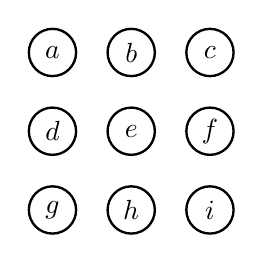
\begin{tikzpicture}
            \def \ax{0}   \def \ay{0}
            \def \bx{1}   \def \by{0}
            \def \cx{2}   \def \cy{0}
            \def \dx{0}   \def \dy{-1}
            \def \ex{1}   \def \ey{-1}
            \def \fx{2}   \def \fy{-1}
            \def \gx{0}   \def \gy{-2}
            \def \hx{1}   \def \hy{-2}
            \def \ix{2}   \def \iy{-2}

            \draw[line width=0.3mm] (\ax, \ay) circle (0.3) node[anchor=center]{$a$};
            \draw[line width=0.3mm] (\bx, \by) circle (0.3) node[anchor=center]{$b$};
            \draw[line width=0.3mm] (\cx, \cy) circle (0.3) node[anchor=center]{$c$};
            \draw[line width=0.3mm] (\dx, \dy) circle (0.3) node[anchor=center]{$d$};
            \draw[line width=0.3mm] (\ex, \ey) circle (0.3) node[anchor=center]{$e$};
            \draw[line width=0.3mm] (\fx, \fy) circle (0.3) node[anchor=center]{$f$};
            \draw[line width=0.3mm] (\gx, \gy) circle (0.3) node[anchor=center]{$g$};
            \draw[line width=0.3mm] (\hx, \hy) circle (0.3) node[anchor=center]{$h$};
            \draw[line width=0.3mm] (\ix, \iy) circle (0.3) node[anchor=center]{$i$};
            % Attacks
            \DrawAttackHorizontal{R}{\ax}{\ay}{\bx}{\by}
            \DrawAttackHorizontal{R}{\dx}{\dy}{\ex}{\ey}
            \DrawAttackHorizontal{R}{\bx}{\by}{\cx}{\cy}
            \DrawAttackVertical{U}{\ex}{\ey}{\bx}{\by}
            \DrawAttackVertical{B}{\ex}{\ey}{\hx}{\hy}
            \DrawAttackHorizontal{L}{\ix}{\iy}{\hx}{\hy}


        \end{tikzpicture}
        \subcaption{\texttt{arg\_amount}=9 \texttt{p}=0.25}
        \label{af:ImplementationGridBasedExampleAFsa}
    \end{subfigure}
    \begin{subfigure}[t]{0.3\textwidth}
    \centering
    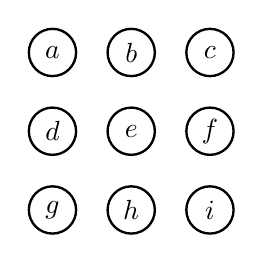
\begin{tikzpicture}
        \def \ax{0}   \def \ay{0}
        \def \bx{1}   \def \by{0}
        \def \cx{2}   \def \cy{0}
        \def \dx{0}   \def \dy{-1}
        \def \ex{1}   \def \ey{-1}
        \def \fx{2}   \def \fy{-1}
        \def \gx{0}   \def \gy{-2}
        \def \hx{1}   \def \hy{-2}
        \def \ix{2}   \def \iy{-2}

        \draw[line width=0.3mm] (\ax, \ay) circle (0.3) node[anchor=center]{$a$};
        \draw[line width=0.3mm] (\bx, \by) circle (0.3) node[anchor=center]{$b$};
        \draw[line width=0.3mm] (\cx, \cy) circle (0.3) node[anchor=center]{$c$};
        \draw[line width=0.3mm] (\dx, \dy) circle (0.3) node[anchor=center]{$d$};
        \draw[line width=0.3mm] (\ex, \ey) circle (0.3) node[anchor=center]{$e$};
        \draw[line width=0.3mm] (\fx, \fy) circle (0.3) node[anchor=center]{$f$};
        \draw[line width=0.3mm] (\gx, \gy) circle (0.3) node[anchor=center]{$g$};
        \draw[line width=0.3mm] (\hx, \hy) circle (0.3) node[anchor=center]{$h$};
        \draw[line width=0.3mm] (\ix, \iy) circle (0.3) node[anchor=center]{$i$};
        % Attacks
        \DrawAttackHorizontal{R}{\ax}{\ay}{\bx}{\by}
        \DrawAttackHorizontal{R}{\dx}{\dy}{\ex}{\ey}
        \DrawAttackHorizontal{R}{\bx}{\by}{\cx}{\cy}
        \DrawAttackHorizontal{L}{\fx}{\fy}{\ex}{\ey}
        \DrawAttackHorizontal{B}{\hx}{\hy}{\gx}{\gy}
        \DrawAttackVertical{U}{\gx}{\gy}{\dx}{\dy}
        \DrawAttackVertical{D}{\cx}{\cy}{\fx}{\fy}
        \DrawAttackVertical{U}{\ex}{\ey}{\bx}{\by}
        \DrawAttackVertical{B}{\ax}{\ay}{\dx}{\dy}
        \DrawAttackVertical{B}{\fx}{\fy}{\ix}{\iy}

    \end{tikzpicture}
    \subcaption{\texttt{arg\_amount}=9 \texttt{p}=0.5}
    \label{af:ImplementationGridBasedExampleAFsb}
\end{subfigure}%
\begin{subfigure}[t]{0.3\textwidth}
    \centering
    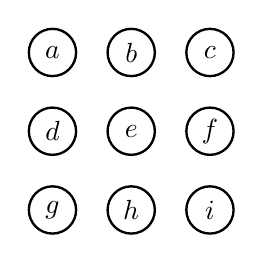
\begin{tikzpicture}
        \def \ax{0}   \def \ay{0}
        \def \bx{1}   \def \by{0}
        \def \cx{2}   \def \cy{0}
        \def \dx{0}   \def \dy{-1}
        \def \ex{1}   \def \ey{-1}
        \def \fx{2}   \def \fy{-1}
        \def \gx{0}   \def \gy{-2}
        \def \hx{1}   \def \hy{-2}
        \def \ix{2}   \def \iy{-2}

        \draw[line width=0.3mm] (\ax, \ay) circle (0.3) node[anchor=center]{$a$};
        \draw[line width=0.3mm] (\bx, \by) circle (0.3) node[anchor=center]{$b$};
        \draw[line width=0.3mm] (\cx, \cy) circle (0.3) node[anchor=center]{$c$};
        \draw[line width=0.3mm] (\dx, \dy) circle (0.3) node[anchor=center]{$d$};
        \draw[line width=0.3mm] (\ex, \ey) circle (0.3) node[anchor=center]{$e$};
        \draw[line width=0.3mm] (\fx, \fy) circle (0.3) node[anchor=center]{$f$};
        \draw[line width=0.3mm] (\gx, \gy) circle (0.3) node[anchor=center]{$g$};
        \draw[line width=0.3mm] (\hx, \hy) circle (0.3) node[anchor=center]{$h$};
        \draw[line width=0.3mm] (\ix, \iy) circle (0.3) node[anchor=center]{$i$};
        % Attacks
        \DrawAttackHorizontal{B}{\bx}{\by}{\ax}{\ay}
        \DrawAttackHorizontal{B}{\ex}{\ey}{\dx}{\dy}
        \DrawAttackHorizontal{B}{\cx}{\cy}{\bx}{\by}
        \DrawAttackHorizontal{B}{\ix}{\iy}{\hx}{\hy}
        \DrawAttackHorizontal{R}{\ex}{\ey}{\fx}{\fy}
        \DrawAttackHorizontal{L}{\hx}{\hy}{\gx}{\gy}
        \DrawAttackVertical{B}{\bx}{\by}{\ex}{\ey}
        \DrawAttackVertical{B}{\fx}{\fy}{\ix}{\iy}
        \DrawAttackVertical{B}{\dx}{\dy}{\gx}{\gy}
        \DrawAttackVertical{D}{\ex}{\ey}{\hx}{\hy}
        \DrawAttackVertical{B}{\ax}{\ay}{\dx}{\dy}
        \DrawAttackVertical{U}{\fx}{\fy}{\cx}{\cy}
    \end{tikzpicture}
    \subcaption{\texttt{arg\_amount}=9 \texttt{p}=0.75}
    \label{af:ImplementationGridBasedExampleAFsc}
\end{subfigure}
\caption{Example AF generated with grid-based approach}
\label{fig:ImplementationGridBasedExampleAFs}
\end{figure}
\vspace{0.3cm}



\paragraph{Level-based} The last algorithm to create concrete AFs we provide, is the level-based approach. The arguments for this script are \texttt{<arg\_amount>}, \texttt{<level>} and \texttt{<p>}. Same as for the grid-based and random-based approach, \texttt{<arg\_amount>} defines how many arguments the computed AF has. The \texttt{<level>} argument restricts the height of the grid to the provided value and \texttt{<p>} is again the probability that an attack between to arguments occurs. The difference to the grid-based approach is the dimension of the grid. While the grid-based approach uses an $n \times n$ grid, in the level-based approach we use a $\texttt{<level>} \times n$ grid. In this context, $n$ is equal to $\lceil \texttt{<arg\_amount>}/\texttt{<level>} \rceil$. An example grid is depicted in \cref{fig:LevelBasedApproach}.


\begin{figure}[h!]
    \centering
    \begin{tikzpicture}
        \def \rectSize{0.7cm}
        \def \rectSpace{0.8cm}

        \foreach \row in {0,1} {
            \foreach \col in {0,1,2,3,4,5,6,7} {
                \def \x{\rectSize * \col + \rectSpace * \col}
                \def \y{\rectSize * \row + \rectSpace * \row}
                \def \xArrowStart{\x+\rectSize/2}
                \def \xArrowEnd{\x+\rectSize/2+\rectSpace}
                \def \yArrowStart{\y+\rectSize/2}
                \def \yArrowEnd{\y+\rectSize/2+\rectSpace}

                % Rectangle
                \node[circle, draw, line width=0.3mm, minimum width=\rectSize, minimum height=\rectSize] at (\x, \y) {};

                \ifnum\col<7
                    % Arrow
                    \draw[dotted,<->, line width=0.3mm, >={To[length=4, width=5]}] (\xArrowStart,\y) -- (\xArrowEnd,\y);
                \fi

                \ifnum\row<1
                    % Arrow
                    \draw[dotted,<->, line width=0.3mm, >={To[length=4, width=5]}] (\x,\yArrowStart) -- (\x,\yArrowEnd);
                \fi
            }
        }
    \end{tikzpicture}
    \caption{Level-based approach with $Level=2$, $Amount=16$ and $p=1$}
    \label{fig:LevelBasedApproach}
\end{figure}


With the level-based approach, we obtain the same structured AF as for the grid-based, but with less neighbours. Every argument can only have $min(\texttt{<level>}+1, 4)$ amount of direct neighbours. This reduces the neighbours even further and thus, decreases the overall computation effort. Example AFs created with the level-based script can be seen in \cref{fig:ImplementationLevelBasedExampleAFs}


\vspace{0.3cm}
\begin{figure}[h]
    \centering
    \begin{subfigure}[t]{0.45\textwidth}
        \centering
        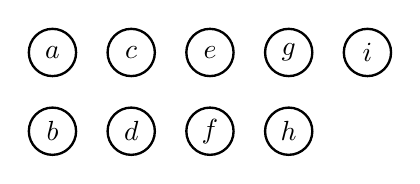
\begin{tikzpicture}
            \def \ax{0}   \def \ay{0}
            \def \bx{0}   \def \by{-1}
            \def \cx{1}   \def \cy{0}
            \def \dx{1}   \def \dy{-1}
            \def \ex{2}   \def \ey{0}
            \def \fx{2}   \def \fy{-1}
            \def \gx{3}   \def \gy{0}
            \def \hx{3}   \def \hy{-1}
            \def \ix{4}   \def \iy{0}

            \draw[line width=0.3mm] (\ax, \ay) circle (0.3) node[anchor=center]{$a$};
            \draw[line width=0.3mm] (\bx, \by) circle (0.3) node[anchor=center]{$b$};
            \draw[line width=0.3mm] (\cx, \cy) circle (0.3) node[anchor=center]{$c$};
            \draw[line width=0.3mm] (\dx, \dy) circle (0.3) node[anchor=center]{$d$};
            \draw[line width=0.3mm] (\ex, \ey) circle (0.3) node[anchor=center]{$e$};
            \draw[line width=0.3mm] (\fx, \fy) circle (0.3) node[anchor=center]{$f$};
            \draw[line width=0.3mm] (\gx, \gy) circle (0.3) node[anchor=center]{$g$};
            \draw[line width=0.3mm] (\hx, \hy) circle (0.3) node[anchor=center]{$h$};
            \draw[line width=0.3mm] (\ix, \iy) circle (0.3) node[anchor=center]{$i$};
            % Attacks
            \DrawAttackHorizontal{R}{\ax}{\ay}{\cx}{\cy}
            \DrawAttackHorizontal{R}{\fx}{\fy}{\hx}{\hy}
            \DrawAttackHorizontal{R}{\dx}{\dy}{\fx}{\fy}
            \DrawAttackHorizontal{L}{\gx}{\gy}{\ex}{\ey}
            \DrawAttackVertical{D}{\ax}{\ay}{\bx}{\by}
            \DrawAttackVertical{B}{\gx}{\gy}{\hx}{\hy}
        \end{tikzpicture}
        \subcaption{\texttt{arg\_amount}=9 \texttt{level}=2 \texttt{p}=0.25}
        \label{af:ImplementationLevelBasedExampleAFsa}
    \end{subfigure}
    \begin{subfigure}[t]{0.45\textwidth}
    \centering
    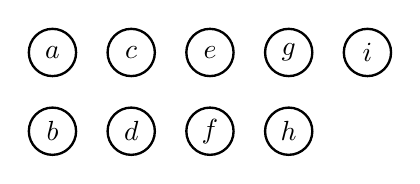
\begin{tikzpicture}
        \def \ax{0}   \def \ay{0}
        \def \bx{0}   \def \by{-1}
        \def \cx{1}   \def \cy{0}
        \def \dx{1}   \def \dy{-1}
        \def \ex{2}   \def \ey{0}
        \def \fx{2}   \def \fy{-1}
        \def \gx{3}   \def \gy{0}
        \def \hx{3}   \def \hy{-1}
        \def \ix{4}   \def \iy{0}

        \draw[line width=0.3mm] (\ax, \ay) circle (0.3) node[anchor=center]{$a$};
        \draw[line width=0.3mm] (\bx, \by) circle (0.3) node[anchor=center]{$b$};
        \draw[line width=0.3mm] (\cx, \cy) circle (0.3) node[anchor=center]{$c$};
        \draw[line width=0.3mm] (\dx, \dy) circle (0.3) node[anchor=center]{$d$};
        \draw[line width=0.3mm] (\ex, \ey) circle (0.3) node[anchor=center]{$e$};
        \draw[line width=0.3mm] (\fx, \fy) circle (0.3) node[anchor=center]{$f$};
        \draw[line width=0.3mm] (\gx, \gy) circle (0.3) node[anchor=center]{$g$};
        \draw[line width=0.3mm] (\hx, \hy) circle (0.3) node[anchor=center]{$h$};
        \draw[line width=0.3mm] (\ix, \iy) circle (0.3) node[anchor=center]{$i$};
        % Attacks
        \DrawAttackHorizontal{B}{\cx}{\cy}{\ax}{\ay}
        \DrawAttackHorizontal{B}{\hx}{\hy}{\fx}{\fy}
        \DrawAttackHorizontal{B}{\ex}{\ey}{\cx}{\cy}
        \DrawAttackHorizontal{B}{\ix}{\iy}{\gx}{\gy}
        \DrawAttackHorizontal{R}{\dx}{\dy}{\fx}{\fy}
        \DrawAttackHorizontal{R}{\ex}{\ey}{\gx}{\gy}
        \DrawAttackHorizontal{L}{\dx}{\dy}{\bx}{\by}
        \DrawAttackVertical{U}{\bx}{\by}{\ax}{\ay}
        \DrawAttackVertical{D}{\gx}{\gy}{\hx}{\hy}
        \DrawAttackVertical{B}{\cx}{\cy}{\dx}{\dy}
        \DrawAttackVertical{B}{\ex}{\ey}{\fx}{\fy}
    \end{tikzpicture}
    \subcaption{\texttt{arg\_amount}=9 \texttt{level}=2 \texttt{p}=0.75}
    \label{af:ImplementationLevelBasedExampleAFsb}
\end{subfigure}%
\caption{Example AF generated with grid-based approach}
\label{fig:ImplementationLevelBasedExampleAFs}
\end{figure}

\paragraph{clustering} The random-based, grid-based and level-based only generate concrete AFs. To be able to generate the abstract AFs based on the concrete ones, we created another independent script. Since clusters make a lot more sense when respecting the locality of the arguments, we cluster arguments which are next to each other (e.g.\ direct neighbours) by traversing the AF via the attacks and adding the argument if we visit it the first time. The size of the cluster is determined on runtime and is a random value between $2$ and the amount of arguments present in the concrete AF.





\section{Usage and Settings}
\label{sec:ImplementationUsageAndSettings}
We implemented the previously mentioned encodings and algorithm into the software called \prog. The tool uses Python as a primary programming language and the library z3 for SAT-Solving. The software is available at

\begin{center}
    \url{https://github.com/p4s3r0/argumentation-framework-clustering}
\end{center}

\noindent
under the MIT license. We provide four different applications, i.e.\ \texttt{SETS}, \texttt{CHECK}, \texttt{CONCRETIZE} and \texttt{FAITHFUL}. Additionally, we need to add the corresponding data via flags, which we can use to change the program's behavior.

\paragraph{Computing extensions} \prog\ can compute all semantics extensions of a given AF. This program can be called with the \texttt{SETS} argument.

\begin{center}
    \texttt{python3 main.py SETS <path\_af>}
\end{center}

The argument \texttt{<path\_af>} is the path to the AF, of which the semantics extensions should be computed. To set the semantics of the extension, check the additional flags in the paragraph below.

\paragraph{Spurious/Faithful check} To check if an abstract AF is faithful or spurious, the program is called with the \texttt{CHECK} argument and followed by the abstract AF and the concrete AF.

\begin{center}
    \texttt{python3 main.py CHECK <path\_abs\_af> -c <path\_con\_af>}
\end{center}

The second argument \texttt{<path\_abs\_af>} is the path to the abstract AF. Next, we add the path to the concrete AF at the \texttt{-c <path\_con\_af>} variable. Furthermore, we can specify the semantics and the algorithm (i.e., BFS or DFS), which is explained in the additional flags paragraph.


\paragraph{Compute faithful AF} If we have a spurious AF and want to compute a faithful abstract AF with only minor transformations, we want to call the program with the \texttt{FAITHFUL} argument.

\begin{center}
    \texttt{python3 main.py FAITHFUL <path\_abs\_af> -c <path\_con\_af> -s <semantics>}
\end{center}

The following arguments are again the path to the abstract AF, followed by the path to the concrete AF. Same as for the previously mentioned programs, the semantics is set with the \texttt{-s <semantics>} flag and the algorithmic approach with the \texttt{-a DFS} or \texttt{-a BFS} flag.

\paragraph{Concretizing arguments} If we want more control over which arguments are concretized to obtain faithfulness, the program must be called with the \texttt{CONCRETIZE} flag.

\begin{center}
    \texttt{python3 main.py CONCRETIZE <path\_abs\_af> -c <path\_con\_af> -p <conc\_args>}
\end{center}

In addition to the abstract and concrete AF paths, we can specify a list of arguments, separated by spaces, to be concretized. The list of arguments \texttt{<conc\_args>} needs to be directly after the \texttt{-p} flag. Additionally, we can use positional arguments like \texttt{-s <semantics>} to specify the semantics or \texttt{-a <alg>} to determine if we want to use BFS or DFS.

\paragraph{Additional Flags} To have complete control of the inner workings of the program and the output printed to the user, we implemented additional flags. The first flag is the semantics flag.

\begin{center}
    \texttt{-s <semantics>}
\end{center}

This argument determines the semantics we are operating on. It is optional for every program and has one of the the following values: \texttt{CF} for conflict-free semantics, which is also the default value, \texttt{AD} for admissible semantics, or \texttt{ST} for stable semantics. 

Next, when executing the program to concretize arguments from a cluster, we need a list of the arguments.

\begin{center}
    \texttt{-p <conc\_args>} 
\end{center}

The arguments that need to be concrete are listed after the \texttt{-p} tag and specified in a joint list separated by spaces.

Furthermore, we can alter the faithful/spurious check algorithm with the \texttt{<alg>} argument.

\begin{center}
    \texttt{-a <alg>}
\end{center}

Here, only two possible values can be selected, i.e., \ the default value \texttt{BFS} and the most of the time more efficient algorithm \texttt{DFS}.

If the refinement of the current semantics is not desired, it can be turned off with the following flag.

\begin{center}
    \texttt{-noref}
\end{center}

We also implemented a visualization of the AFs, which can be triggered using the following flag.

\begin{center}
    \texttt{-vis}
\end{center}

The visualization will show the abstract AF and the concrete AF if they are part of the program call. Finally, it will show the resulting AF. To ''spectate`` the current computation and have more insight into the algorithm, we can add the \texttt{-verbose} flag. This will print interim findings to the user directly while calculating.


\subsection{Input Format}
The input format for the AFs has a clear structure and is divided into four parts: i.e.\ $header$, $attacks$, $orphans$ and $clusters$. The optional parts (i.e., $orphans$ and $clusters$) are introduced with the \texttt{--<name>--} tag. Each tag is defined and the usage of the part is explained in the corresponding paragraph. If an optional part is empty, e.g.\ we have a concrete AF without clusters, we can simply omit the part by not including the tag. The singletons and clusters need to be indexed consecutively with positive integers, i.e., letters and symbols are not allowed.

\paragraph{Header} The header is the first line of the input file and is the unique ''p-line``. Here we specify the amount of singletons \texttt{<n>} present in the AF.

\vspace{0.3cm}
\begin{center}
    \texttt{p af <n>}
\end{center}
\vspace{0.3cm}

The amount \texttt{<n>} does not include the amount of clusters from the specific AF and has to be a positive integer greater than $0$. The abstracted arguments that are clustered are not included in the amount \texttt{<n>} as well.

\paragraph{Attacks} Next, we define the attacks of the AF. Every attack is defined on a unique line and consists of a source \texttt{<s>} and a target \texttt{<t>}, which are the numerical indices of the arguments where \texttt{<s>} attacks \texttt{<t>}.

\vspace{0.3cm}
\begin{center}
    \texttt{<s1> <t1>}\\
    \texttt{<s2> <t2>}\\
    \texttt{<s3> <t3>}\\
    \texttt{<s4> <t4>}
\end{center}
\vspace{0.3cm}



\paragraph{Orphans} If an argument is not referenced in the attacks, i.e.\ the argument does not attack any other argument and is not attacked by any other argument, we call it an orphan. Orphans are not required coercively and are defined in the orphans section with the \texttt{--attackless--} tag. Every orphan is defined on a unique line and is the numerical indices of the argument.

\vspace{0.3cm}
\begin{center}
    \hspace{2.25cm}
    \makebox[0pt]{%
        \parbox{5cm}{% Adjust the width as necessary
            \texttt{--attackless--}\\
            \texttt{<a1>}\\
            \texttt{<a2>}\\
            \texttt{<a3>}\\
            \texttt{<a4>}
        }
    }
\end{center}
\vspace{0.3cm}



\paragraph{Clusters} The next optional part are the clusters. The tag is the \texttt{--cluster--} tag and each cluster is defined by a numerical positive integer and the indices of the arguments that are inside the cluster.

\vspace{0.3cm}
\begin{center}
    \hspace{1cm}
    \makebox[0pt]{%
        \parbox{5cm}{% Adjust the width as necessary
            \texttt{--cluster--}\\
            \texttt{<c1> <- <a1> <a2> <a3>}
            \texttt{<c2> <- <a4> <a5> <a6>}
            \texttt{<c3> <- <a7> <a8> <a9>}
        }
    }
\end{center}
\vspace{0.3cm}

The cluster \texttt{<c>} is followed by an arrow pointing to the cluster \texttt{<-}, followed by a list of argument indeces separated by spaces.

\paragraph{Comments} Finally, we can use comment lines. A comment is marked as such, with a hashtag \texttt{\#} at the beginning of the line. Every character followed by the hastag is ignored by the parser.

\vspace{0.3cm}
\begin{center}
    \texttt{\# This is a comment}
\end{center}
\vspace{0.3cm}


\begin{example}
    Let us define $\hat{G}=(\hat{A}, \hat{R})$ to be an abstract AF depicted in \cref{af:implementationInputExample}, with the arguments $\hat{A}=\{a, b, c, \hat{h}\}$ where the cluster $\hat{h}$ contains the arguments $d$, $e$ and $f$. The attacks of the cluster are defined as $\hat{R}=\big\{ (a, b), (\hat{h}, b), (\hat{h}, \hat{h})\big\}$.

\vspace{0.3cm}
\begin{figure}[h]
    \centering
    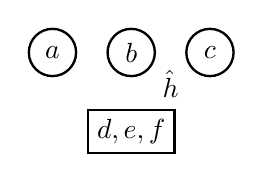
\begin{tikzpicture}
        % Singletons
        \def \ax{0}     \def \ay{0}
        \def \bx{1}     \def \by{0}
        \def \cx{2}     \def \cy{0}
        \def \hx{1}     \def \hy{-1}

        \node[rectangle, draw, line width=0.3mm] at (\hx, \hy) {$d, e, f$};
        \node at (\hx+0.5, \hy+0.6) {$\hat{h}$};
        \draw[line width=0.3mm] (\ax, \ay) circle (0.3) node[anchor=center]{$a$};
        \draw[line width=0.3mm] (\bx, \by) circle (0.3) node[anchor=center]{$b$};
        \draw[line width=0.3mm] (\cx, \cy) circle (0.3) node[anchor=center]{$c$};

        % Attacks
        \DrawSelfAttackLeftTopCluster{\hx-0.45}{\hy + 0.3}
        \DrawAttackHorizontal{R}{\ax}{\ay}{\bx}{\by}
        \DrawAttackVertical{U}{\hx}{\hy}{\bx}{\by}
    \end{tikzpicture}
    \caption{Abstract AF $\hat{G}$}
    \label{af:implementationInputExample}
\end{figure}

\vspace{0.3cm}
We can translate the AF into the following input format. The arguments are mapped to numerical positive numbers, i.e., $a \rightarrow 1$, $b \rightarrow 2$, $c \rightarrow 3$, $d \rightarrow 4$, $e \rightarrow 5$, $f \rightarrow 6$ and $\hat{h} \rightarrow 7$.

\vspace{0.3cm}
\begin{center}
    \fbox{%
        \parbox{5cm}{% Adjust the width as necessary
            \texttt{p af 3}\\
            \texttt{\# This is a comment}\\
            \texttt{1 2}\\
            \texttt{7 2}\\
            \texttt{7 7}\\
            \texttt{--attackless--}\\
            \texttt{3}\\
            \texttt{--cluster--}\\
            \texttt{7 <- 4 5 6}
        }
    }
\end{center}
\end{example}
